\section{Luck runs out in the new shaft series}

\subsection{What a Coincidence}
There were plenty of deep leads now, with the continuation of Blue Danube at the bottom or halfway down (into what would be Upside Down Chamber) and the enticing passage in the opposite direction that I’d briefly scouted on the previous trip. I felt I’d done quite well in terms of big finds, and Rhys was keen to pick up where we left off so instead I took Kenneth to explore the SE extension of Colony.
 
We had got as far as Mighty Fine Indeed when disaster struck. I had just descended the first pitch and called ‘Rope Free’ when I was struck by something falling from above. For a fraction of a second I assumed I was dead, my head smashed open by a rock, but as I staggered and collapsed I realised I was inexplicably still alive. I screamed and swore as my vision danced, and as the stars faded I looked around. Sitting next to me was the drill, in its bag. The drill was meant to be clipped to Kenneth, yet here it was. Now my swearing had a more precise target, and I began to really get into it. I imagine Kenneth apologised, or at least tried to, but I wasn’t really listening. When he reached the ground we had a little chat about the importance of clipping the bag carefully to your harness. Rhys and Arun were below us and had heard all the commotion, so I told them we were ‘fine, just fine’ and continued on.
 
After pausing to giggle in terror at Tanguy’s Terrible Pitch in Hall of the Mountain King, we pushed on, quickly reaching the cairn I’d placed the previous day. The route on was quite easy, with a climb up through a boulder choke and a bit of scrambling at different levels. At one point, thick brown mud filled the entire hading rift, forcing a flat out crawl which lasted a few metres.
 
Kenneth lead the way, following a faint draft, and soon we arrived at a dead end - the passage turned into a descending phreatic which was filled with loose, flakey rock. I dug for a bit whilst Kenneth searched for a way on, but it seemed hopeless and I thought our luck had run out. Then Kenneth called from behind me that he had found the way on. I paused for the moment, remembering some words from our website: “Perhaps more poignantly, when you discover passageway that reaches a dead-end; you may well be the last person to ever visit that particular place in the world.”
 
Turning and climbing back up, I saw Kenneth’s lead. It was another flat out crawl in a tight, mud filled rift. This one required a sideways undulation for a few metres to a very small chamber that lead to an ascending phreatic. At the top of this, the phreatic dropped sharply at an angle of around 60’ to the horizontal. Somewhat worried that we’d be unable to get back up, we plunged down, reaching a low, wide mud filled chamber at the bottom.
 
Most of the chamber was taken up by a deep pit, and on the far wall there was a passage leading off. We carefully picked our way round the pit and into the continuing passage. The passage was a classic keyhole shape of a phreatic circle with a vadose extension below, but here the vadose section was very narrow and deep, less than a welly across but several metres down. A trickle of water ran at the bottom down to the big pit, and mostly came from a drippy aven we discovered halfway along the passage. The passage was very straight, with a well defined bend in the middle, and we raced up it to see where it lead.
 
At the far end was a small, sandy chamber. On the left wall was a window into a big chamber, and the right wall lead up a steep, muddy slope. We’d left the drill behind so we decided to push as far as we could before resorting to bolting. The steep muddy slope had the ceiling very close above, and and after a few failed attempts to get up, we settled on climbing up as if it were an overhang, using the muddy floor for support and the ceiling for handholds.
 
Near the top I discovered something puzzling - dark red squares of material, clearly artificial but very unclear as to their nature. Clambering up the last of the slope lead to a window into a big chamber with an ICCC rope dropping straight passed. We weren’t sure about the age or state of the bolts, and decided not to use these ropes. The ledge was littered with the dark red squares, which defied our careful examination. Kenneth named the passage ‘What a Coincidence’ as we’d reached the old shaft series in a neat, straight line.
 
At this point we needed to get the drill, which we’d cleverly left all the way back near the Hall of the Mountain King, far from what was now the pushing front. We went back, and found that the climb up the steep phreatic wasn’t too terrible, and retrieved the drill and ropes. We rigged a traverse around the deep pit (but didn’t descend it as we wanted to link up with the parallel shaft series) and then Kenneth put a y-hang in the window at the end of the passage. He descended all the way down, but this caused massive rope rub. I descended to the top of a big pile of boulders, and found it was possible to scramble down to the floor, which avoided the rope rub.
 
The chamber was wide and large. A blue and white rope came down the far wall. We could see a traverse line leading off at the top, but there was otherwise very little clue where we were. We explored a little, confirming that there was a way on, but with so much still to survey we had to turn back at this point.
 
Our survey confirmed that we were near the old shaft series (which starts at TTT), but we couldn’t find any PSS to tie into, and there must be a large error somewhere to place us over 40 m away from the most probable lead. Clare and Tanguy believe they saw our rope on the far side of a chamber when they went down the TTT route, so one goal for 2017 is to resolve this ambiguity. And there’s still the undescended deep pit with the trickle of water in the middle of What a Coincidence, and a potential deep camp spot amongst the insulating mud.
 
 
\name{Jack and Kenneth}

\subsection{Tight and Scrotty and Gambler’s Ruin}
 
Jack, Rhys, Clare and Miriam
 
An elite team comprising of three former presidents (Clare, Rhys, Jack) and one novice (Miriam) headed off to properly kill Upside Down Chamber and Blue Danube. At the top of Blue Danube we split up - I went down Upide Down Chamber to de-rig and re-rig down Blue Danube, and Rhys started bolting over the top of Blue Danube to a continuation of Colony on the far side. Clare and Miriam went to check out Fratnik’s shit lead, a rift coming off at the Colony/Hall of the Mountain King.
 
I came back out of Upside Down Chamber and chatted to Rhys before heading back along Colony to see how Miriam and Clare were getting on. They responded to my ‘ey-oh’, but said something was wrong. I dropped through the rift and found them - Miriam had fallen a very short distance and her ankle was tender. We waited for a bit and had some food and water, and decided to keep caving. The lead was practically dead - it seems to be a boulder collapse that follows underneath Colony. There is some potential.
 
Back at Rhys’ Folly, and Rhys had admitted his folly. The tube on the far side merely reconnected back into Blue Danube, and his epic traverse (many bolts placed from a horizontal position, supported by cowstails) was at an end. We had one lead left - the stream at the bottom of Blue Danube.
 
 \begin{figure*}[t!]
\checkoddpage \ifoddpage \forcerectofloat \else \forceversofloat \fi
   \centering
     \begin{subfigure}[t]{0.627\textwidth}
        \centering
        \frame{\includegraphics[width=\linewidth]{"images/2016/jack-end-2016/Top_of_Upside_Down__1_".jpg}}
        \caption{} \label{Top of Upside Down}
    \end{subfigure}
    \hfill
         \begin{subfigure}[t]{0.353\textwidth}
        \centering
        \frame{\includegraphics[width=\linewidth]{"images/2016/jack-end-2016/Rhys-folly__1_".jpg}}
        \caption{} \label{Rhys on traverse}
    \end{subfigure}
    \caption{
    \emph{a} Clare and Miriam peering over the edge at the end of \emph{Colony}. 
    \emph{b} Rhys's Folly, a bold traverse into a phreatic tube which reconnects with \emph{Upside Down Chamber} --- Rhys Tyers}
\end{figure*}
 
 
We descended down the clean washed, pale grey shaft and quickly eased into the rift below to avoid the spray. The first pitch was short, and I rigged it off naturals. Then the rift opened out, the water dropped away below and we found ourself in a small chamber with a window looking back into Upside Down Chamber. Disappointing. There was still one way on, going out into Upside Down Chamber and then swinging back through another window into another chamber, its floor filled with boulders. We pushed all the leads we could, which were all Tight and Scrotty, hence the name. Even Clare decided nothing was going, so we surveyed our way out.
 
At this point, desperation or inspiration struck. What if Rhys and Arun’s lead at the bottom of Upside Down Chamber wasn’t truly dead? We dropped into the chamber and climbed up the boulder slope. In the process I stood on the bat skeleton, which had been guarded by the world’s worst cairn. Sorry bat.
 
The rift down was sharp and unpleasant. We were short on rope. Rhys rigged down on bolts he’d placed the previous day, and we wriggled down vertically, enjoying the scraping sensation on all our soft squishy parts. At the bottom was a narrow rift crawl, just as sharp as everything else. We cleared lots of rocks from it, then Rhys and Clare squeezed through and passed more rocks back to me. At this point it was large enough even for me to get through, but Rhys and Clare had found a pitch so I was sent back up for the drill and bolts.
 
Back at the bottom, the tension was palpable. There was a good draft and an open pitch. We had so little rope that at the bottom of the 3 m pitch we cut the rope a good metre off the ground. Miriam was eyeing us with increasing wariness - this was the infamous cave lust she’d heard so much about. Between us, Miriam and I built a take off cairn so that we could actually get back onto the rope. She was unimpressed by the innovation.
 
Rhys and Clare were already bolting the next pitch. It had one bolt. The back up was happy thoughts. The pitch head was one of the tightest I’ve ever done, and I doubted I’d get back through. At the bottom the cave was clearly very dead. The only possible way on was in the ceiling, about 3 m up. The draft is good, but it looks like it’s flowing through a huge fault, rather than a true cave. The rock is just shattered, rather than eroded by water. A very odd place.

\begin{figure*}[h]
\checkoddpage \ifoddpage \forcerectofloat \else \forceversofloat \fi
\centering
\frame{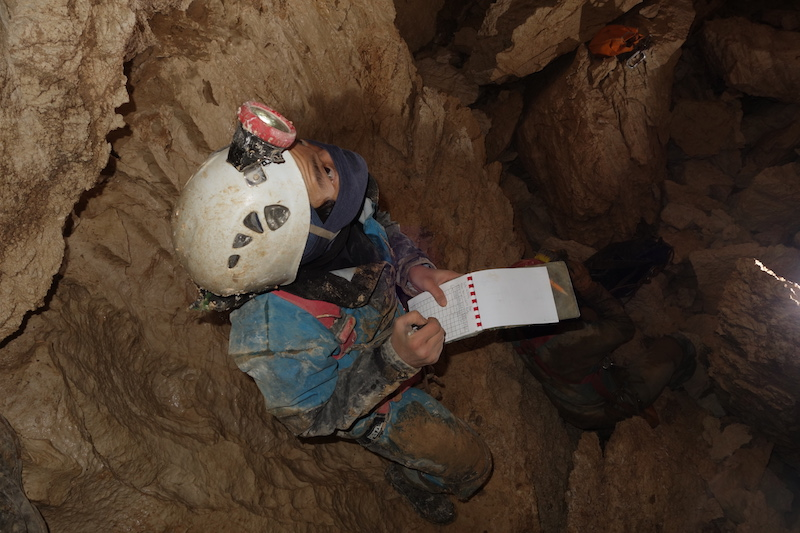
\includegraphics[width=\textwidth]{images/2016/jack-end-2016/Survey-Clare-2016.jpg}}
\caption{Clare surveying in Upside Down chamber after 'killing' a hopeless dig --- Rhys Tyers}
\label{Tight}
\end{figure*}
 
We’d taken every chance we could, and eventually we’d run out of luck and met our Gambler’s Ruin (a random walk in one or two dimensions visit every point with probability unity, leading to a gambler with finite money always going bust eventually). We surveyed out, squeezing through a rift that ruined several oversuits, and began the long climb to the surface. We had reached the deepest point of the expedition this year.
 
 
Why Man Here
 
Rhys and Jack
 
With only one day of caving left, Rhys and I were keen to squeeze as much exploration in as possible. Our first target was the rift which Knot Very Good enters - Rhys had spotted a window, and got to work bolting his way around to it (unperturbed by Rhys’ Folly going nowhere on his previous pushing trip). The window turned out to be a large solution pocket, but on the far wall he spotted another window. As we were short on bolts, this was left un-pushed and we ascended, looking for easier leads.
 
In the long, winding rift between Sane and Sober and Knot Very Good Rhys had spotted a way down. The rift has many false floors, and passages follow at all levels. We dropped down at Station 11 (named after the PSS) and found a chamber with a false floor. In one direction, up-rift, I reconnected with the large chamber next to Sane and Sober where the lower Monatip connection enters. In the down rift direction we did a sketchy traverse on a sloping ledge, and found a small, beautiful chattière that was too tight to continue.
 
We returned to the main branch, and climbed up into the roof. There is a higher level passage here that has many flat out crawls through fine sand. This popped out half way up a chamber. The floor was a boulder collapse and we couldn’t get through to a chamber that took all of our light. Half way up the chamber was a chattière that seemed to go. Desperate at this point, we grabbed rocks from the floor and smashed away at the obstructions. This gave us enough space to wriggle through, and we followed the passage until it popped out facing the small hand-line pitch between Sane and Sober and Knot Very Good. Drat.
 
We returned to the upper level passage, despondent, when Rhys spotted a small, grim looking chute heading off. He struggled through and declared it was lovely. As I squeezed in I realised quite how tight it was, but Rhys kindly moved a big rock from the floor and I managed to slither through. We were in a tight, sharp rift. We quickly go to the upper end, which tightened down, but with some hammering could go. 
 
We then descended in the rift. The rock was brutally sharp and tore off chunks of flesh and oversuit. At the bottom, we found a very small (two person sized) chamber, filled with rocks. We started to excavate, piling rocks back along our escape route. Soon we had cleared enough space to see that there was a way on into a vast chamber. We grabbed the drill and began to bolt, lifting out rocks with tape and smashing others with the bolting hammer. I squeezed through and into a large space. Dropping down, I placed a deviation and continue to a broad ledge, strewn with rocks. In the distance I could see the rope of Knot Very Good - yet another blasted connection!
 
Our exploration of the rift, and indeed the sistem, was at an end for this year. Dejected, but eager to return we headed out. The rift is interesting, but it is unlikely there are any real leads here, as the water seems to have followed the simplest path many times, twisting and returning to its theme like a slow and ponderous fugue of water and rock.
